%
%

%%-----------------------------------------------------
%%-----------------------------------------------------
\usebackgroundtemplate{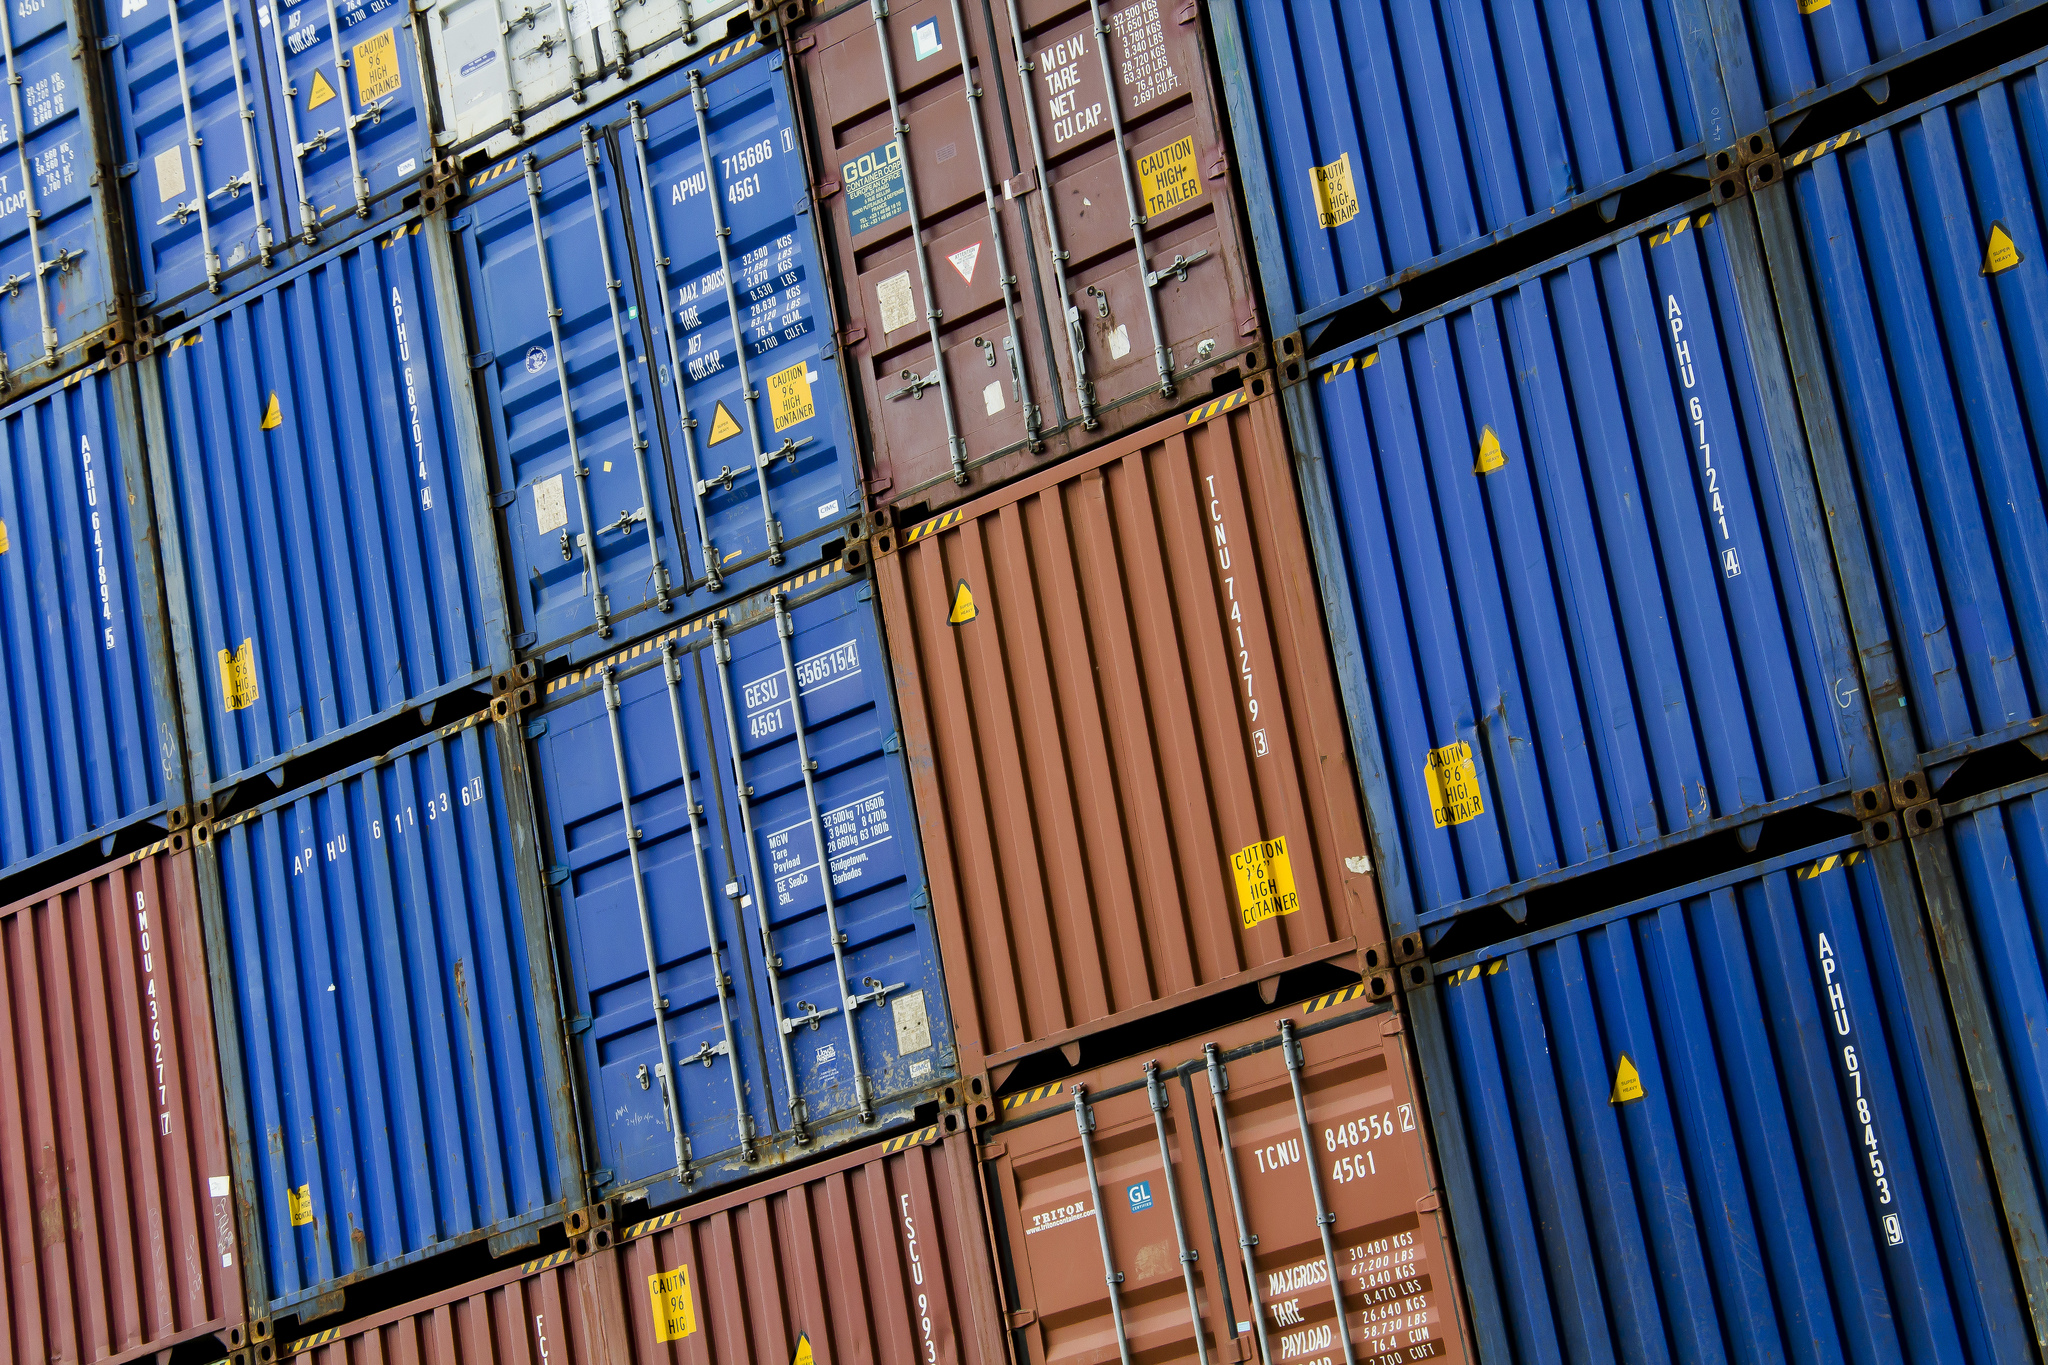
\includegraphics[width=\paperwidth,height=\paperheight]{figs/docker-containers.jpg}}
% Original figure: Flickr, Luke Price, ``Containers, Port of Rotterdam'', CC-by 2.0
% https://www.flickr.com/photos/lukeprice88/9703431992
{\bf
  \textcolor[rgb]{1,1,1}{
    \section{Contenedores por todas partes}
  }
}

\usebackgroundtemplate{}

%%-----------------------------------------------------
\begin{frame}
\frametitle{Contenedores software}

\begin{columns}[T]
\begin{column}{.48\textwidth}
{\Large
  \begin{itemize}
  \item Virtualización sobre sistema operativo
  \item Evolución de la idea de chroot
  \item Aislamiento \\
    (disco, memoria) \\
  \item Gestión de recursos
  \end{itemize}
}
\end{column}%
\hfill%
\begin{column}{.40\textwidth}
{\Large
  \begin{itemize}
  \item Más ligero que máquinas virtuales completas
  \item Mismo kernel \\
    que host \\
  \item Docker, LXC, LXD, \\
    FreeBSD Jail... \\
\end{itemize}
}
\end{column}%
\end{columns}

\end{frame}


%%-----------------------------------------------------
\begin{frame}
\frametitle{Docker (search trend)}

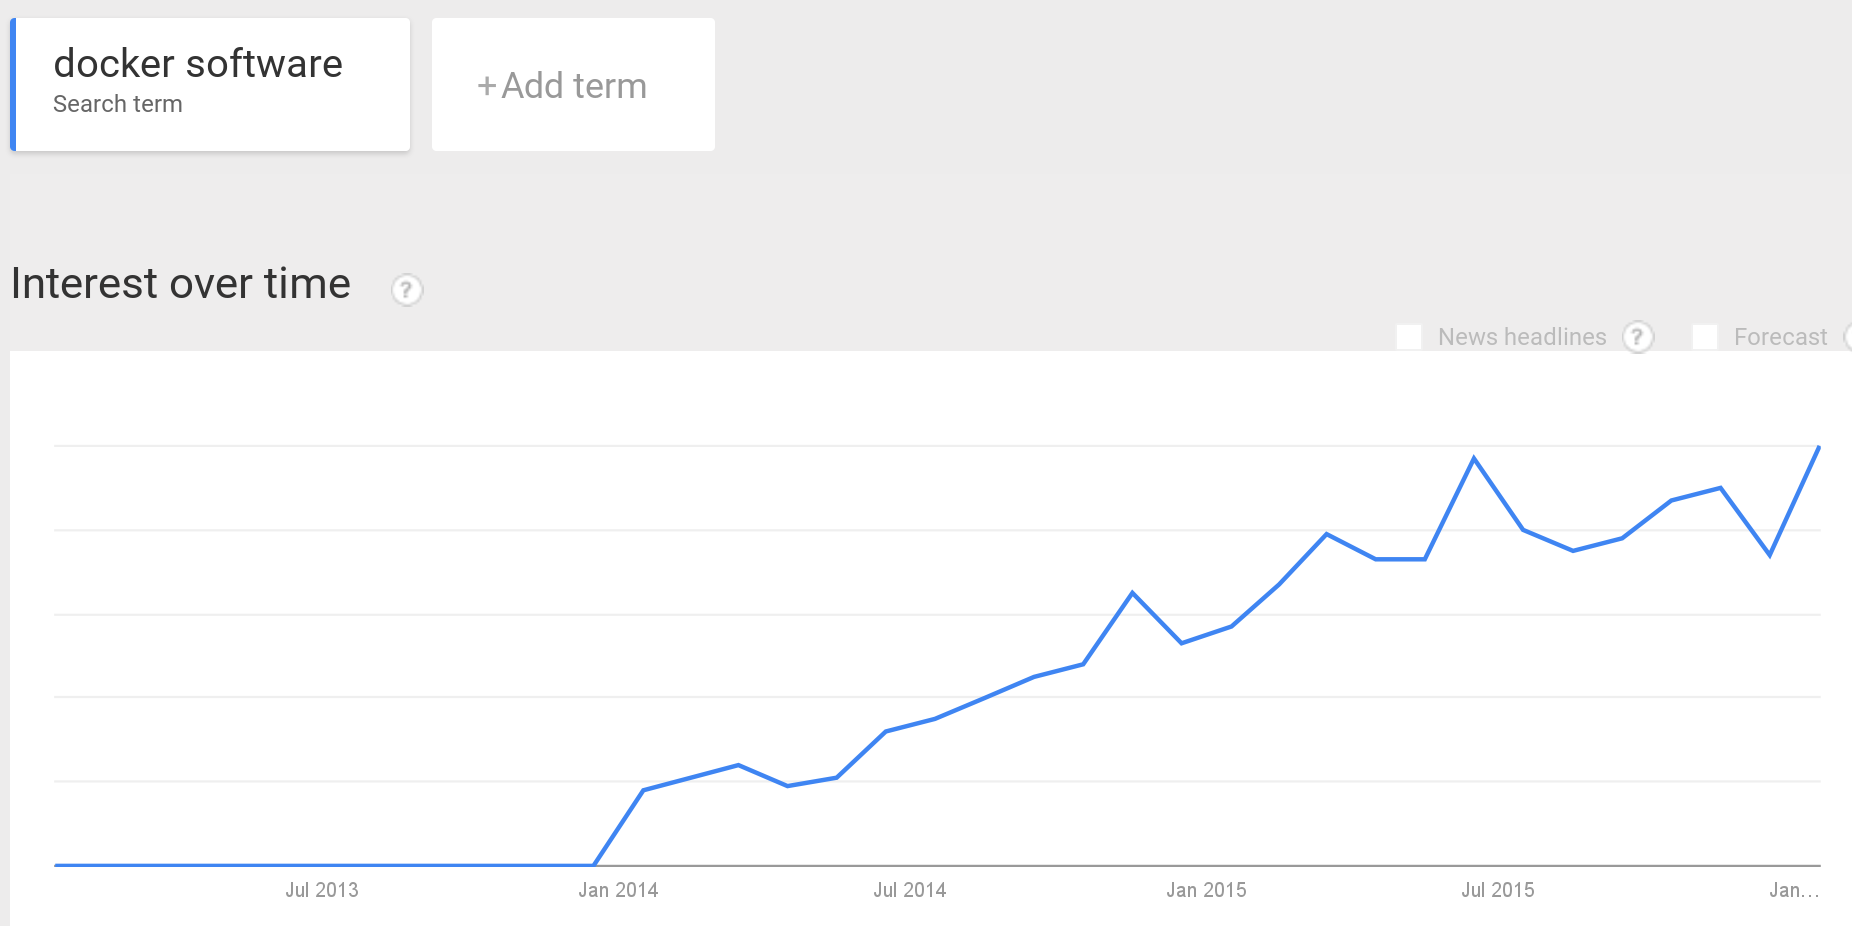
\includegraphics[width=12cm]{figs/docker-trend}


\end{frame}

%%-----------------------------------------------------
\begin{frame}
\frametitle{Docker}


\includegraphics[width=7cm]{figs/docker-logo}

\begin{columns}[T]
\begin{column}{.38\textwidth}

\begin{flushright}
{\Large
  \url{http://docker.com} 

  \vspace{1cm}

  \url{http://hub.docker.com/}
}
\end{flushright}

\end{column}%
\hfill%
\begin{column}{.60\textwidth}
{\Large
\begin{itemize}
\item Automatización del despliegue de aplicaciones en contenedores software
\item Montado sobre cgroups \\ (gestión de recursos), \\
  namespaces \\ (separación de recursos), \\
  sistema de ficheros con unión \\
\end{itemize}
}
\end{column}%
\end{columns}

\end{frame}

%%-----------------------------------------------------
\begin{frame}
\frametitle{Referencias y enlaces}

\begin{flushright}
  Luke Price, ``Containers, Port of Rotterdam'', CC-by 2.0 \\
  \url{https://www.flickr.com/photos/lukeprice88/9703431992} \\
\end{flushright}  

\end{frame}






